% !LW recipe = latexmk (xelatex)
% RenalLens, adapted from poster_template/main.tex (UChicago CS / Gemini v1.1.0).
% In this directory: latexmk -xelatex -jobname=RenalLens_Poster main.tex
% The supplied Gemini theme uses the Raleway and Lato font families.
\documentclass[final]{beamer}

\usepackage[T1]{fontenc}
\usepackage{lmodern}
\usepackage[size=custom,width=132,height=80,scale=1.0]{beamerposter}
\usetheme{gemini}
\usecolortheme{uchicago}
\usepackage{graphicx}
\usepackage[patch=none]{microtype}
\usepackage{tikz}
\usepackage{pgfplots}
\pgfplotsset{compat=1.18}
\usepackage{anyfontsize}
\pdfstringdefDisableCommands{\def\translate#1{#1}}
\setlength{\abovecaptionskip}{1ex}

% Substitute the CityUHK palette in the template's existing color roles.
\definecolor{maroon}{HTML}{941344}
\definecolor{red}{HTML}{D2133F}
\definecolor{violet}{HTML}{681132}
\definecolor{lightgray}{HTML}{F6E5EA}
\definecolor{darkgray}{HTML}{615961}
\setbeamercolor{block example title}{parent=block title}
\setbeamercolor{block example separator}{parent=block separator}

\newlength{\sepwidth}
\newlength{\flowcolwidth}
\newlength{\colwidth}
\setlength{\sepwidth}{0.0175\paperwidth}
\setlength{\flowcolwidth}{0.47375\paperwidth}
\setlength{\colwidth}{0.31\paperwidth}
\newcommand{\separatorcolumn}{\begin{column}{\sepwidth}\end{column}}

\title{RenalLens: When Missing Data Change the Picture}
\author{BAI Yingdong \and CHEN Canyang \and LI Jiaheng \and PENG Peiyan \and ZHAI Junsong \and ZHANG Junjie}
\institute[CityUHK]{Chronic kidney disease data \enspace\textbar\enspace DSC5002-C61, Group 65}
\hypersetup{pdftitle={RenalLens: When Missing Data Change the Picture},
  pdfauthor={BAI Yingdong, CHEN Canyang, LI Jiaheng, PENG Peiyan, ZHAI Junsong, ZHANG Junjie},
  pdfsubject={DSC5002 RenalLens group project}}
\footercontent{
  \href{https://doi.org/10.24432/C5G020}{UCI Chronic Kidney Disease \enspace doi:10.24432/C5G020} \hfill
  RenalLens \enspace --- \enspace DSC5002, C61 Group 65 \hfill
  \href{https://doi.org/10.48550/arXiv.2609.00065}{Figure methods \enspace Kassis et al. (2026)} \hfill
  \href{https://github.com/CanyonChen/RenalLens}{github.com/CanyonChen/RenalLens}}

\begin{document}
\addtobeamertemplate{headline}{}
{
  \begin{tikzpicture}[remember picture,overlay]
    \node [anchor=north east, inner sep=3cm] at ([xshift=0.0cm,yshift=2.5cm]current page.north east)
      {
\includegraphics[height=8.0cm]{../CityUHK_Logo_2.png}};
  \end{tikzpicture}
}

\begin{frame}[t]
\begin{columns}[t]
\separatorcolumn

\begin{column}{\flowcolwidth}
  \begin{block}{Start with Record 43}
    \begin{tabular*}{\linewidth}{@{\extracolsep{\fill}}lr@{}}
Urine albumin & \textbf{Grade 0} \\[0.3ex]
Diabetes history & \textbf{No} \\[0.3ex]
Creatinine & \textbf{1.0 mg/dL} \\[0.3ex]
Hemoglobin & \textbf{9.7 (UCI units)} \\[0.3ex]
Recorded anemia & \textbf{Yes} \\[0.3ex]
Random glucose & \textbf{\color{maroon}204 mg/dL} \\[0.3ex]
\end{tabular*}


    \textbf{One CKD-labeled record; only the red cell assessment (rbc) is missing.}
    The 24-field rule excludes it; the five-marker rule retains its measured 204 mg/dL glucose.
  \end{block}
\end{column}

\separatorcolumn

\begin{column}{\flowcolwidth}
  \begin{alertblock}{Compare three processing choices}
    \textbf{Available:} use the measured fields each question needs.\par
    \textbf{Complete:} require all 24 explanatory fields; compare a five-marker rule.\par
    \textbf{Filled:} use pooled numeric medians and categorical modes, without diagnosis labels.
  \end{alertblock}
\end{column}

\separatorcolumn
\end{columns}
\vspace{.4ex}
\begin{columns}[t]
\separatorcolumn

\begin{column}{\colwidth}
  \begin{block}{1. Deletion changes who remains}
    \begin{figure}
      \centering
      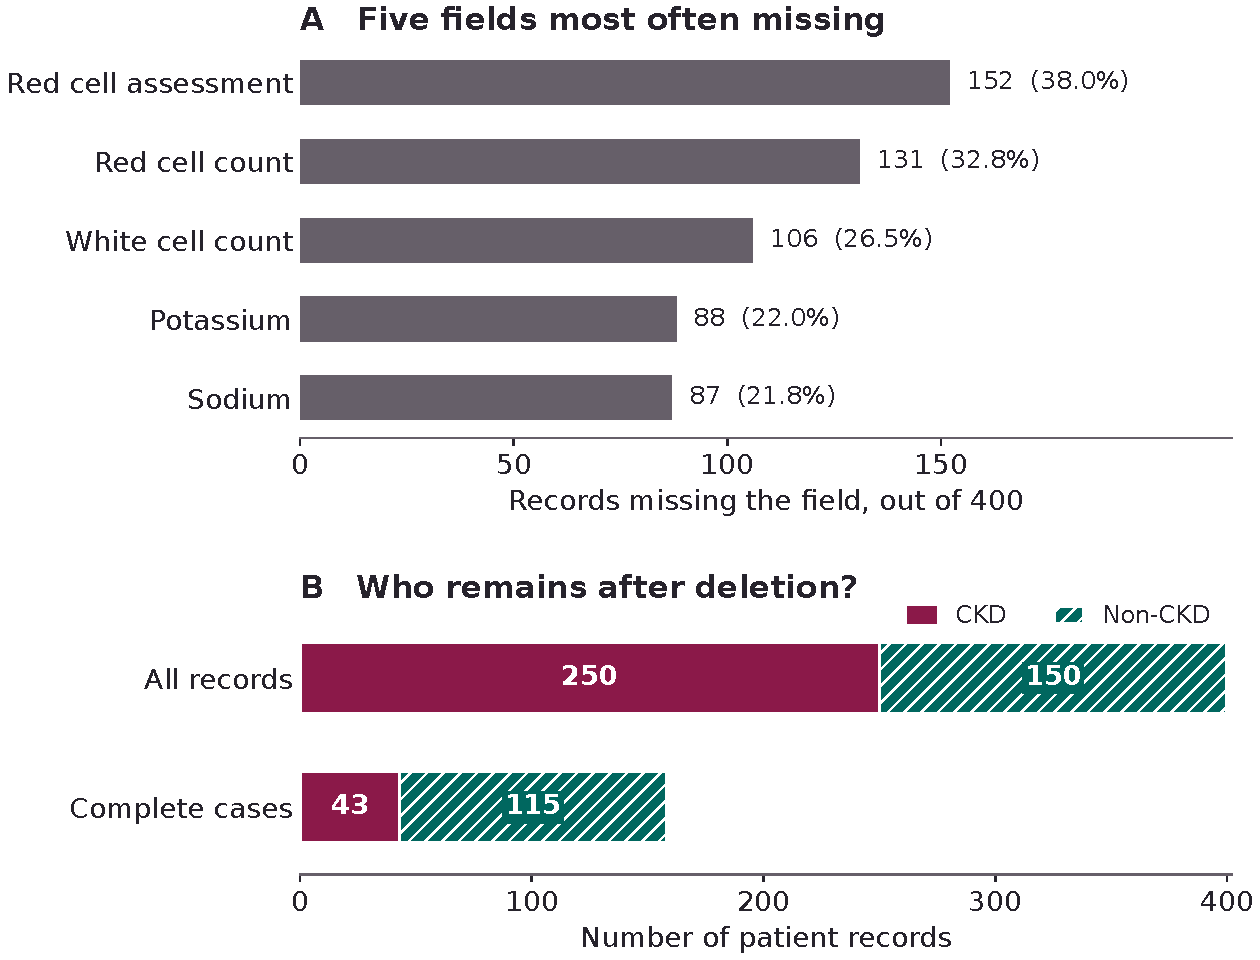
\includegraphics[width=\linewidth]{figures/cohort_selection.pdf}
      \caption{Five markers: hemoglobin, creatinine, urea, glucose and blood pressure. Counts share one zero-based axis; percentages give CKD shares.}
    \end{figure}
    \textbf{CKD retention: 43/250 with 24 fields, versus 165/250 with five.}
    Non-CKD retention is 115/150 versus 135/150.

    \begin{figure}
      \centering
      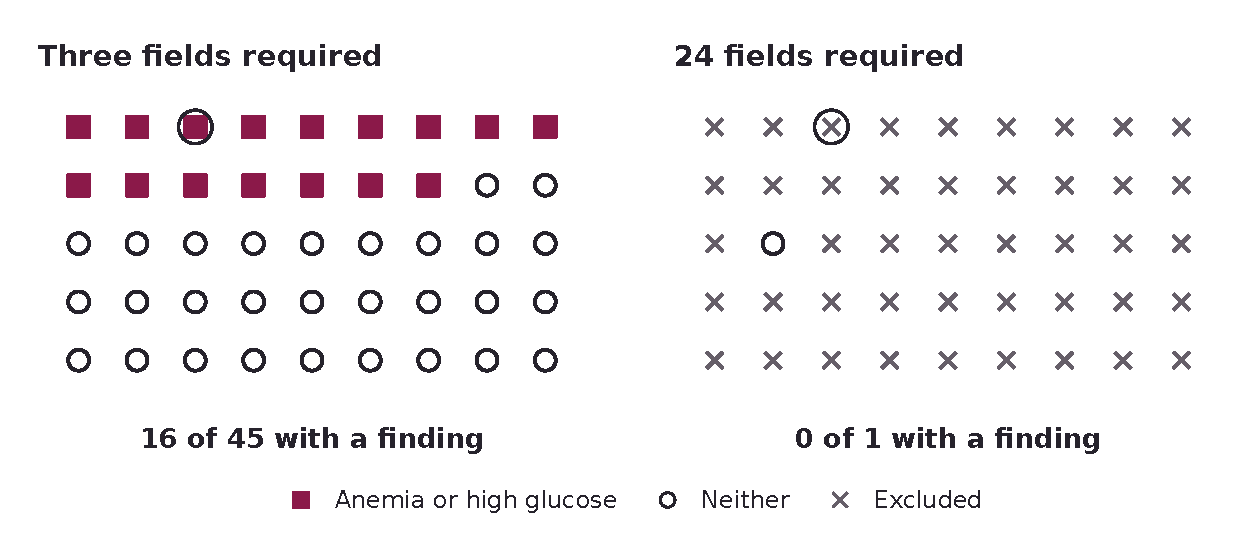
\includegraphics[width=\linewidth]{figures/grade_zero_selection.pdf}
      \caption{The same 45 grade-0 CKD patients have observed albumin, anemia status and glucose. Positions preserve patient identity; the ring marks Record 43. A finding means anemia or glucose $\geq$200 mg/dL.}
    \end{figure}
    \textbf{Only 1/45 remains; all 16 with a finding are excluded.}

    Under the 24-field rule, median creatinine changes in opposite directions: \textbf{1.30 to 1.10 mg/dL}
    overall ($n=383\to158$), but \textbf{2.25 to 4.10} within CKD
    ($n=238\to43$). Selection changes both diagnosis mix and patients within each group.
  \end{block}
\end{column}

\separatorcolumn

\begin{column}{\colwidth}
  \begin{block}{2. Filling creates a spike at 12.65}
    \textbf{52/400 records (13\%)} receive the same hemoglobin value.
    \begin{figure}
      \centering
      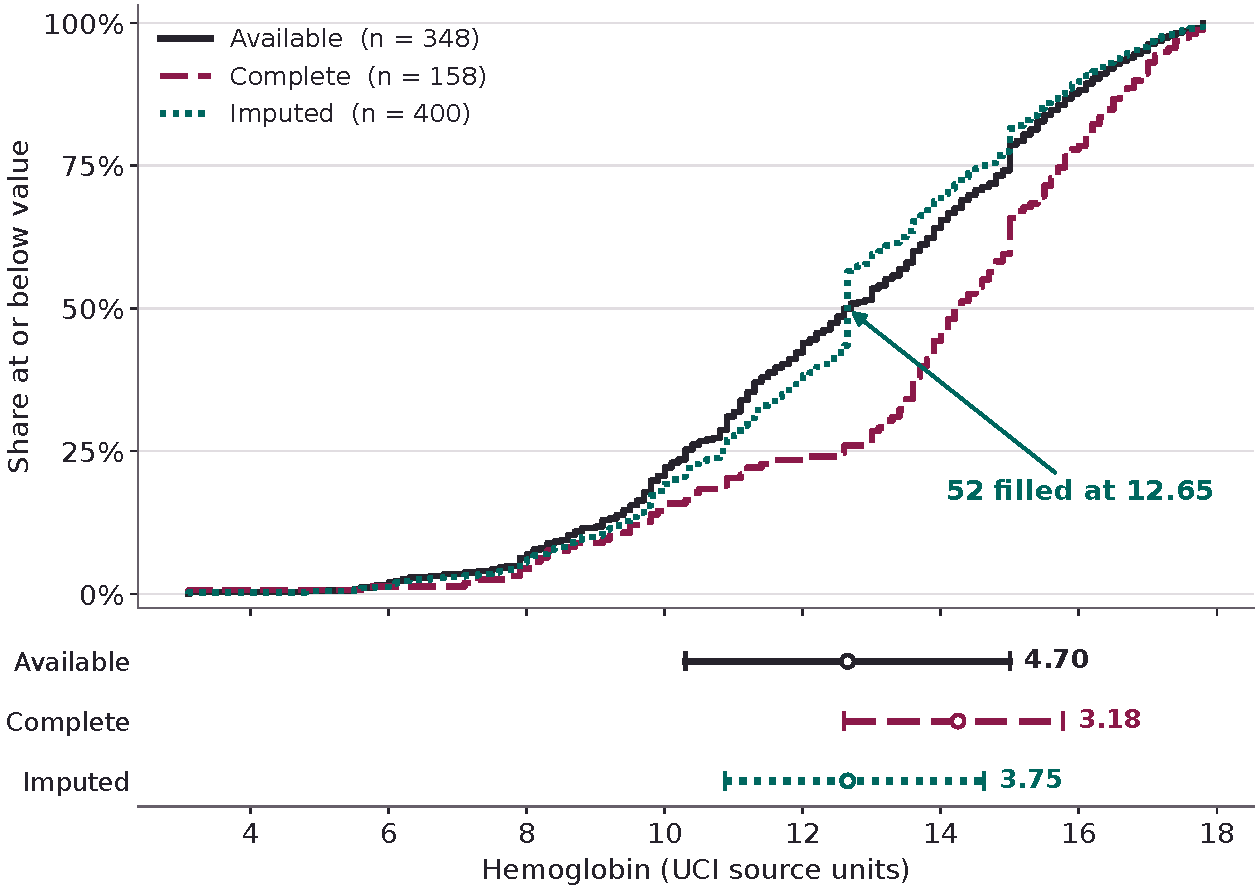
\includegraphics[width=\linewidth]{figures/hemoglobin_views.pdf}
      \caption{Curves show the share at or below each value. None of the 348 measured values equals 12.65. Hemoglobin keeps UCI's source units.}
    \end{figure}
  \end{block}

  \begin{block}{3. Complete cases exceed the glucose bound}
    \textbf{46.5\% in the selected 43, versus at most 44.0\% in all 250.}
    \begin{figure}
      \centering
      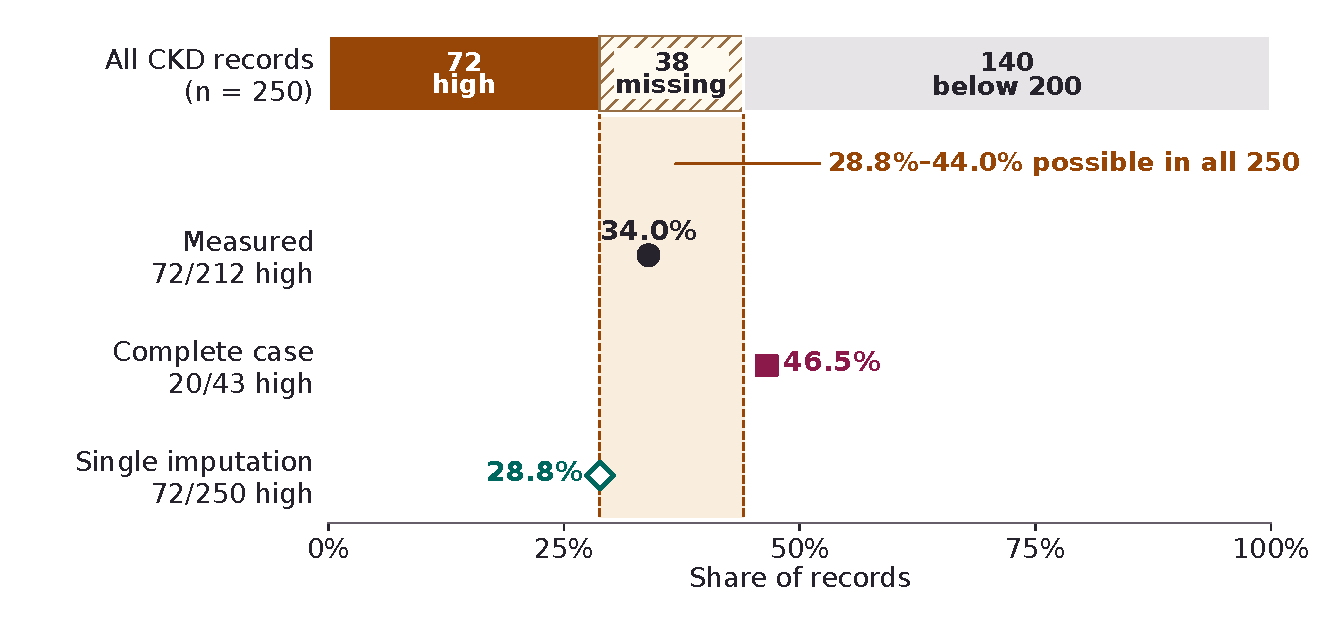
\includegraphics[width=\linewidth]{figures/glucose_bounds.pdf}
      \caption{High means glucose $\geq$200 mg/dL. The band assigns all 38 missing readings as low or high: 72/250 to 110/250. These are logical bounds, not confidence intervals. Each point prints its own denominator.}
    \end{figure}
  \end{block}
\end{column}

\separatorcolumn

\begin{column}{\colwidth}
  \begin{block}{4. Deletion changes the association}
    Creatinine and blood urea give different answers about linear and rank association after deletion.
    \begin{figure}
      \centering
      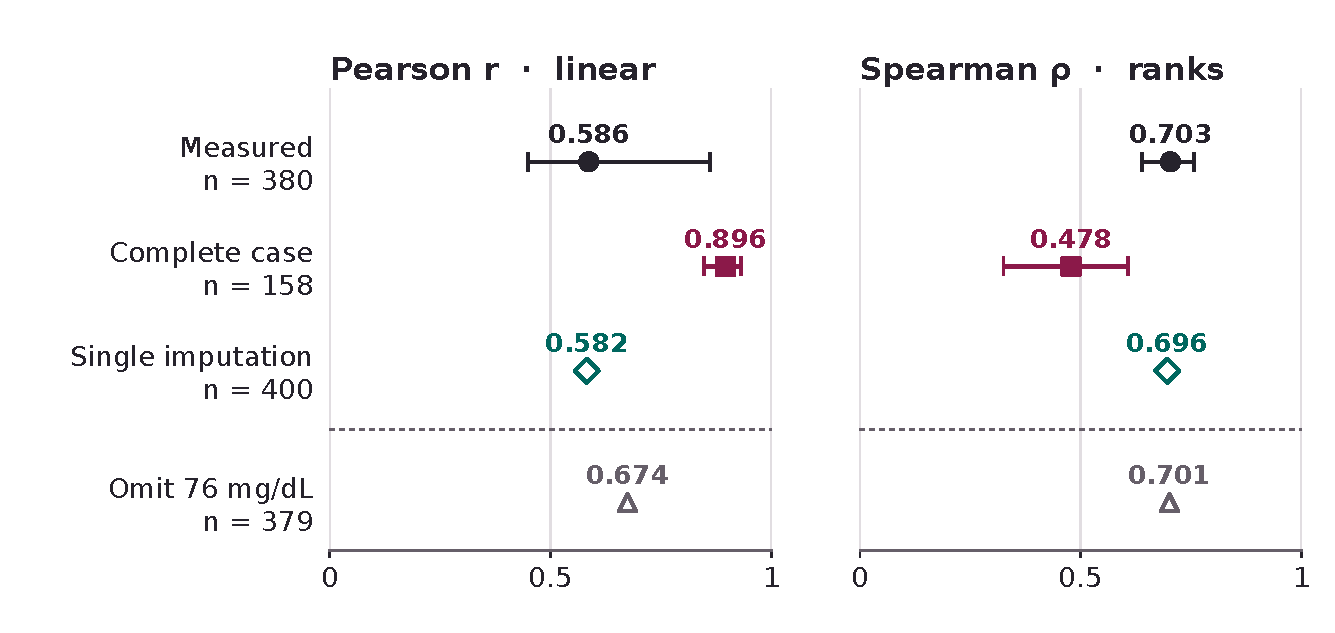
\includegraphics[width=\linewidth]{figures/renal_coefficients.pdf}
      \caption{Whiskers: 95\% bootstrap intervals from 5,000 resamples within diagnosis. Filled estimates are descriptive. The last row separately omits the highest creatinine from measured pairs.}
    \end{figure}
    \textbf{Pearson rises from 0.586 to 0.896; Spearman falls from 0.703 to 0.478.} The highest creatinine (76 mg/dL) mainly affects the linear result; it remains in the main analysis.
  \end{block}

  \begin{block}{5. Units change the summary}
    Hold the same 400 filled records and five markers fixed; change only their measurement scales.
    \begin{figure}
      \centering
      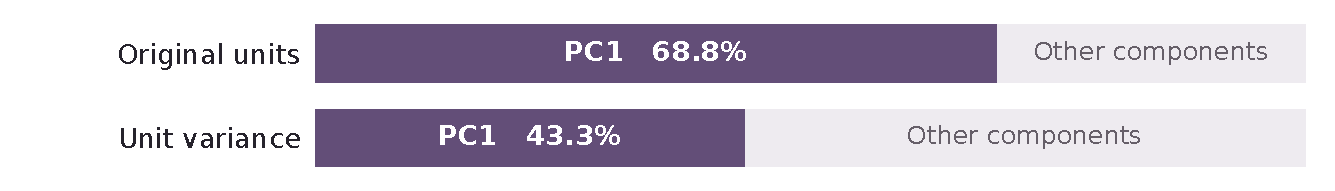
\includegraphics[width=\linewidth]{figures/pca_scale.pdf}
      \caption{Signed PC1 coefficients use the same coefficient scale. Standardization moves the axis from glucose dominance to urea, hemoglobin and creatinine, with hemoglobin pointing oppositely.}
    \end{figure}
    \textbf{Show each denominator; distinguish measured values from filled values.}
  \end{block}
\end{column}

\separatorcolumn
\end{columns}
\end{frame}
\end{document}
